\documentclass[12pt,a4paper]{article}

\usepackage[margin=2.5cm]{geometry}
\setlength{\headheight}{14pt}
\usepackage{graphicx}
\usepackage{booktabs}
\usepackage{array}
\usepackage{tabularx}
\usepackage{amsmath}
\usepackage{parskip}
\usepackage{titlesec}
\usepackage{fancyhdr}
\usepackage{enumitem}
\usepackage{microtype}
\usepackage{float}
\usepackage{listings}
\usepackage{caption}
\usepackage{url}
\usepackage[hidelinks]{hyperref}

\lstset{
    basicstyle=\ttfamily\small,
    breaklines=true,
    frame=single,
    numbers=left,
    numberstyle=\tiny,
    numbersep=8pt,
    captionpos=b
}

\titleformat{\section}{\large\bfseries}{\thesection}{1em}{}[\vspace{-0.3em}\rule{\textwidth}{0.4pt}]
\titleformat{\subsection}{\normalsize\bfseries}{\thesubsection}{1em}{}

\pagestyle{fancy}
\fancyhf{}
\fancyhead[L]{\small\textit{RTT Live Monitor --- Mini Project Report}}
\fancyhead[R]{\small\textit{CN SEM VI}}
\fancyfoot[C]{\small\thepage}
\renewcommand{\headrulewidth}{0.4pt}

\begin{document}

\begin{titlepage}
    \centering
    \vspace*{2cm}

    {\Large \textbf{Department of Computer Engineering}}\\[0.3em]
    {\large Third Year B.Tech --- Semester VI}\\[0.5em]
    {\large Computer Networks (Mini Project)}

    \vspace{1.5cm}
    \rule{\textwidth}{1.5pt}\\[0.4em]
    {\LARGE \textbf{Real-Time TCP Round-Trip Time}}\\[0.3em]
    {\LARGE \textbf{(RTT) Monitoring Tool}}\\[0.4em]
    \rule{\textwidth}{1.5pt}

    \vspace{1.5cm}
    \begin{tabular}{ll}
        \textbf{Author:}   & Malhar Falke \\[0.3em]
        \textbf{Roll No.:} & [Your Roll No.] \\[0.3em]
        \textbf{Date:}     & April 2026 \\[0.3em]
        \textbf{Repo:}     & \url{https://github.com/malharc373/rtt_monitor}
    \end{tabular}

    \vfill
    {\large \textit{Submitted in partial fulfilment of the requirements\\
    for the degree of Bachelor of Technology}}
\end{titlepage}

\tableofcontents
\newpage

\section{Abstract}

This project implements a real-time TCP Round-Trip Time (RTT) monitoring tool
using Python and Scapy. The tool passively sniffs TCP SYN/ACK handshakes on a
live network interface, computes per-flow RTT values, and categorises traffic
by port and protocol. Results are reported at configurable intervals on the
terminal and saved as a CSV file and a multi-panel analysis chart on completion.

Three versions were developed iteratively (v1--v3), each adding new capabilities.
Three live capture sessions on a college WiFi network captured a combined
\textbf{446 RTT samples} over 60-second windows. Results confirm consistent
median RTT under 1\,ms for HTTPS traffic, with P90 values below 12\,ms.

\section{Introduction}

Round-Trip Time (RTT) is a fundamental Quality-of-Service metric in
computer networks. It measures the time for a data packet to travel from a
source host to a destination and back. High or variable RTT leads to poor user
experience in real-time applications such as video conferencing and interactive
web services.

Traditional RTT measurement injects active probe packets, such as ICMP ping,
into the network. This project instead uses a \textbf{passive approach} by
observing real TCP traffic and matching SYN and SYN-ACK timestamps.

\subsection{Passive vs Active Monitoring}

\begin{table}[H]
    \centering
    \caption{Comparison of RTT monitoring approaches}
    \begin{tabularx}{\textwidth}{lXX}
        \toprule
        \textbf{Aspect} & \textbf{Active} & \textbf{Passive} \\
        \midrule
        Traffic overhead & Injects packets & No extra traffic \\
        Firewall issues & ICMP may be blocked & Uses existing TCP flows \\
        Realism & Synthetic & Real user traffic \\
        Setup & Simple & Needs raw socket access \\
        \bottomrule
    \end{tabularx}
\end{table}

\section{Objectives}

\begin{enumerate}[leftmargin=*]
    \item Capture live TCP RTT samples by passively sniffing SYN/SYN-ACK pairs.
    \item Compute Mean, P50, P90, P95 and Max RTT per window.
    \item Categorise traffic by type or port.
    \item Display live interval-based RTT summaries on the terminal.
    \item Save CSV and PNG outputs automatically on session completion.
    \item Support offline analysis of pre-captured \texttt{.pcap} files.
\end{enumerate}

\section{System Design and Architecture}

The tool works as a passive packet observer. It intercepts raw Ethernet frames,
filters TCP packets, and matches SYN and SYN-ACK packets by 4-tuple flow key to
compute RTT.

\subsection{RTT Formula}

\[
\text{RTT} = t_{\text{SYN-ACK}} - t_{\text{SYN}}
\]

In v2, an additional DATA-ACK method was used for better coverage:

\[
\text{RTT}_{\text{DATA-ACK}} = t_{\text{ACK}} - t_{\text{DATA}}
\]

\subsection{Pipeline}

\begin{enumerate}[leftmargin=*]
    \item Scapy sniffer captures raw TCP packets on the network interface.
    \item Flow tracker maps each 4-tuple to its SYN timestamp.
    \item SYN-ACK arrival completes the RTT measurement for that flow.
    \item pandas aggregates per-category statistics at each time window.
    \item matplotlib generates the final multi-panel PNG chart.
\end{enumerate}

\section{Version-wise Development}

\subsection{v1 --- Baseline Live Monitor}

v1 established the first working RTT monitor. It performed live packet sniffing,
classified traffic into three categories (LAN, Campus WiFi, Remote Internet),
and generated CSV summaries and a four-panel chart.

\textbf{Main characteristics:}
\begin{itemize}[leftmargin=*]
    \item Live-only operation
    \item 3 traffic categories
    \item Basic congestion spike detection using $2.5\times$ median threshold
    \item Hardcoded output path
\end{itemize}

\subsection{v2 --- Offline pcap Analysis}

v2 introduced offline analysis of a real packet capture file. It improved flow
coverage by supporting both SYN-SYNACK and DATA-ACK RTT estimation.

\textbf{Main characteristics:}
\begin{itemize}[leftmargin=*]
    \item Reads \texttt{real/capture.pcap}
    \item Dual RTT measurement methods (SYN-ACK and DATA-ACK)
    \item Generates per-category and per-flow statistics
\end{itemize}

\subsection{v3 --- Configurable Live Monitor (Final)}

v3 is the final and most polished version. It supports configurable intervals
and duration through command-line arguments and prints per-window statistics
during capture.

\begin{lstlisting}[language=bash, caption={Example v3 command}]
sudo python3 projectv3.py --live --interval 5 --duration 60
\end{lstlisting}

\textbf{Main improvements over v1 and v2:}
\begin{itemize}[leftmargin=*]
    \item Fully configurable via \texttt{--interval} and \texttt{--duration} flags
    \item Live terminal dashboard printed every N seconds
    \item Fixed missing \texttt{P95\_ms} column in live aggregation path
    \item Saves \texttt{rtt\_live.csv} and \texttt{rtt\_analysis.png} on completion
\end{itemize}

\section{Results and Analysis}

\subsection{v1 Results}

\begin{table}[H]
    \centering
    \caption{v1 per-category RTT summary (all values in ms)}
    \begin{tabular}{lrrrrrr}
        \toprule
        \textbf{Category} & \textbf{N} & \textbf{Mean} & \textbf{P50} & \textbf{P90} & \textbf{P95} & \textbf{Max} \\
        \midrule
        LAN (Wired)     & 779 & 1.441  & 1.219  & 1.810  & 2.063   & 14.351  \\
        Campus WiFi     & 846 & 15.058 & 9.448  & 36.819 & 60.791  & 131.137 \\
        Remote Internet & 618 & 66.400 & 46.145 & 70.453 & 248.383 & 511.843 \\
        \bottomrule
    \end{tabular}
\end{table}

\begin{figure}[H]
    \centering
    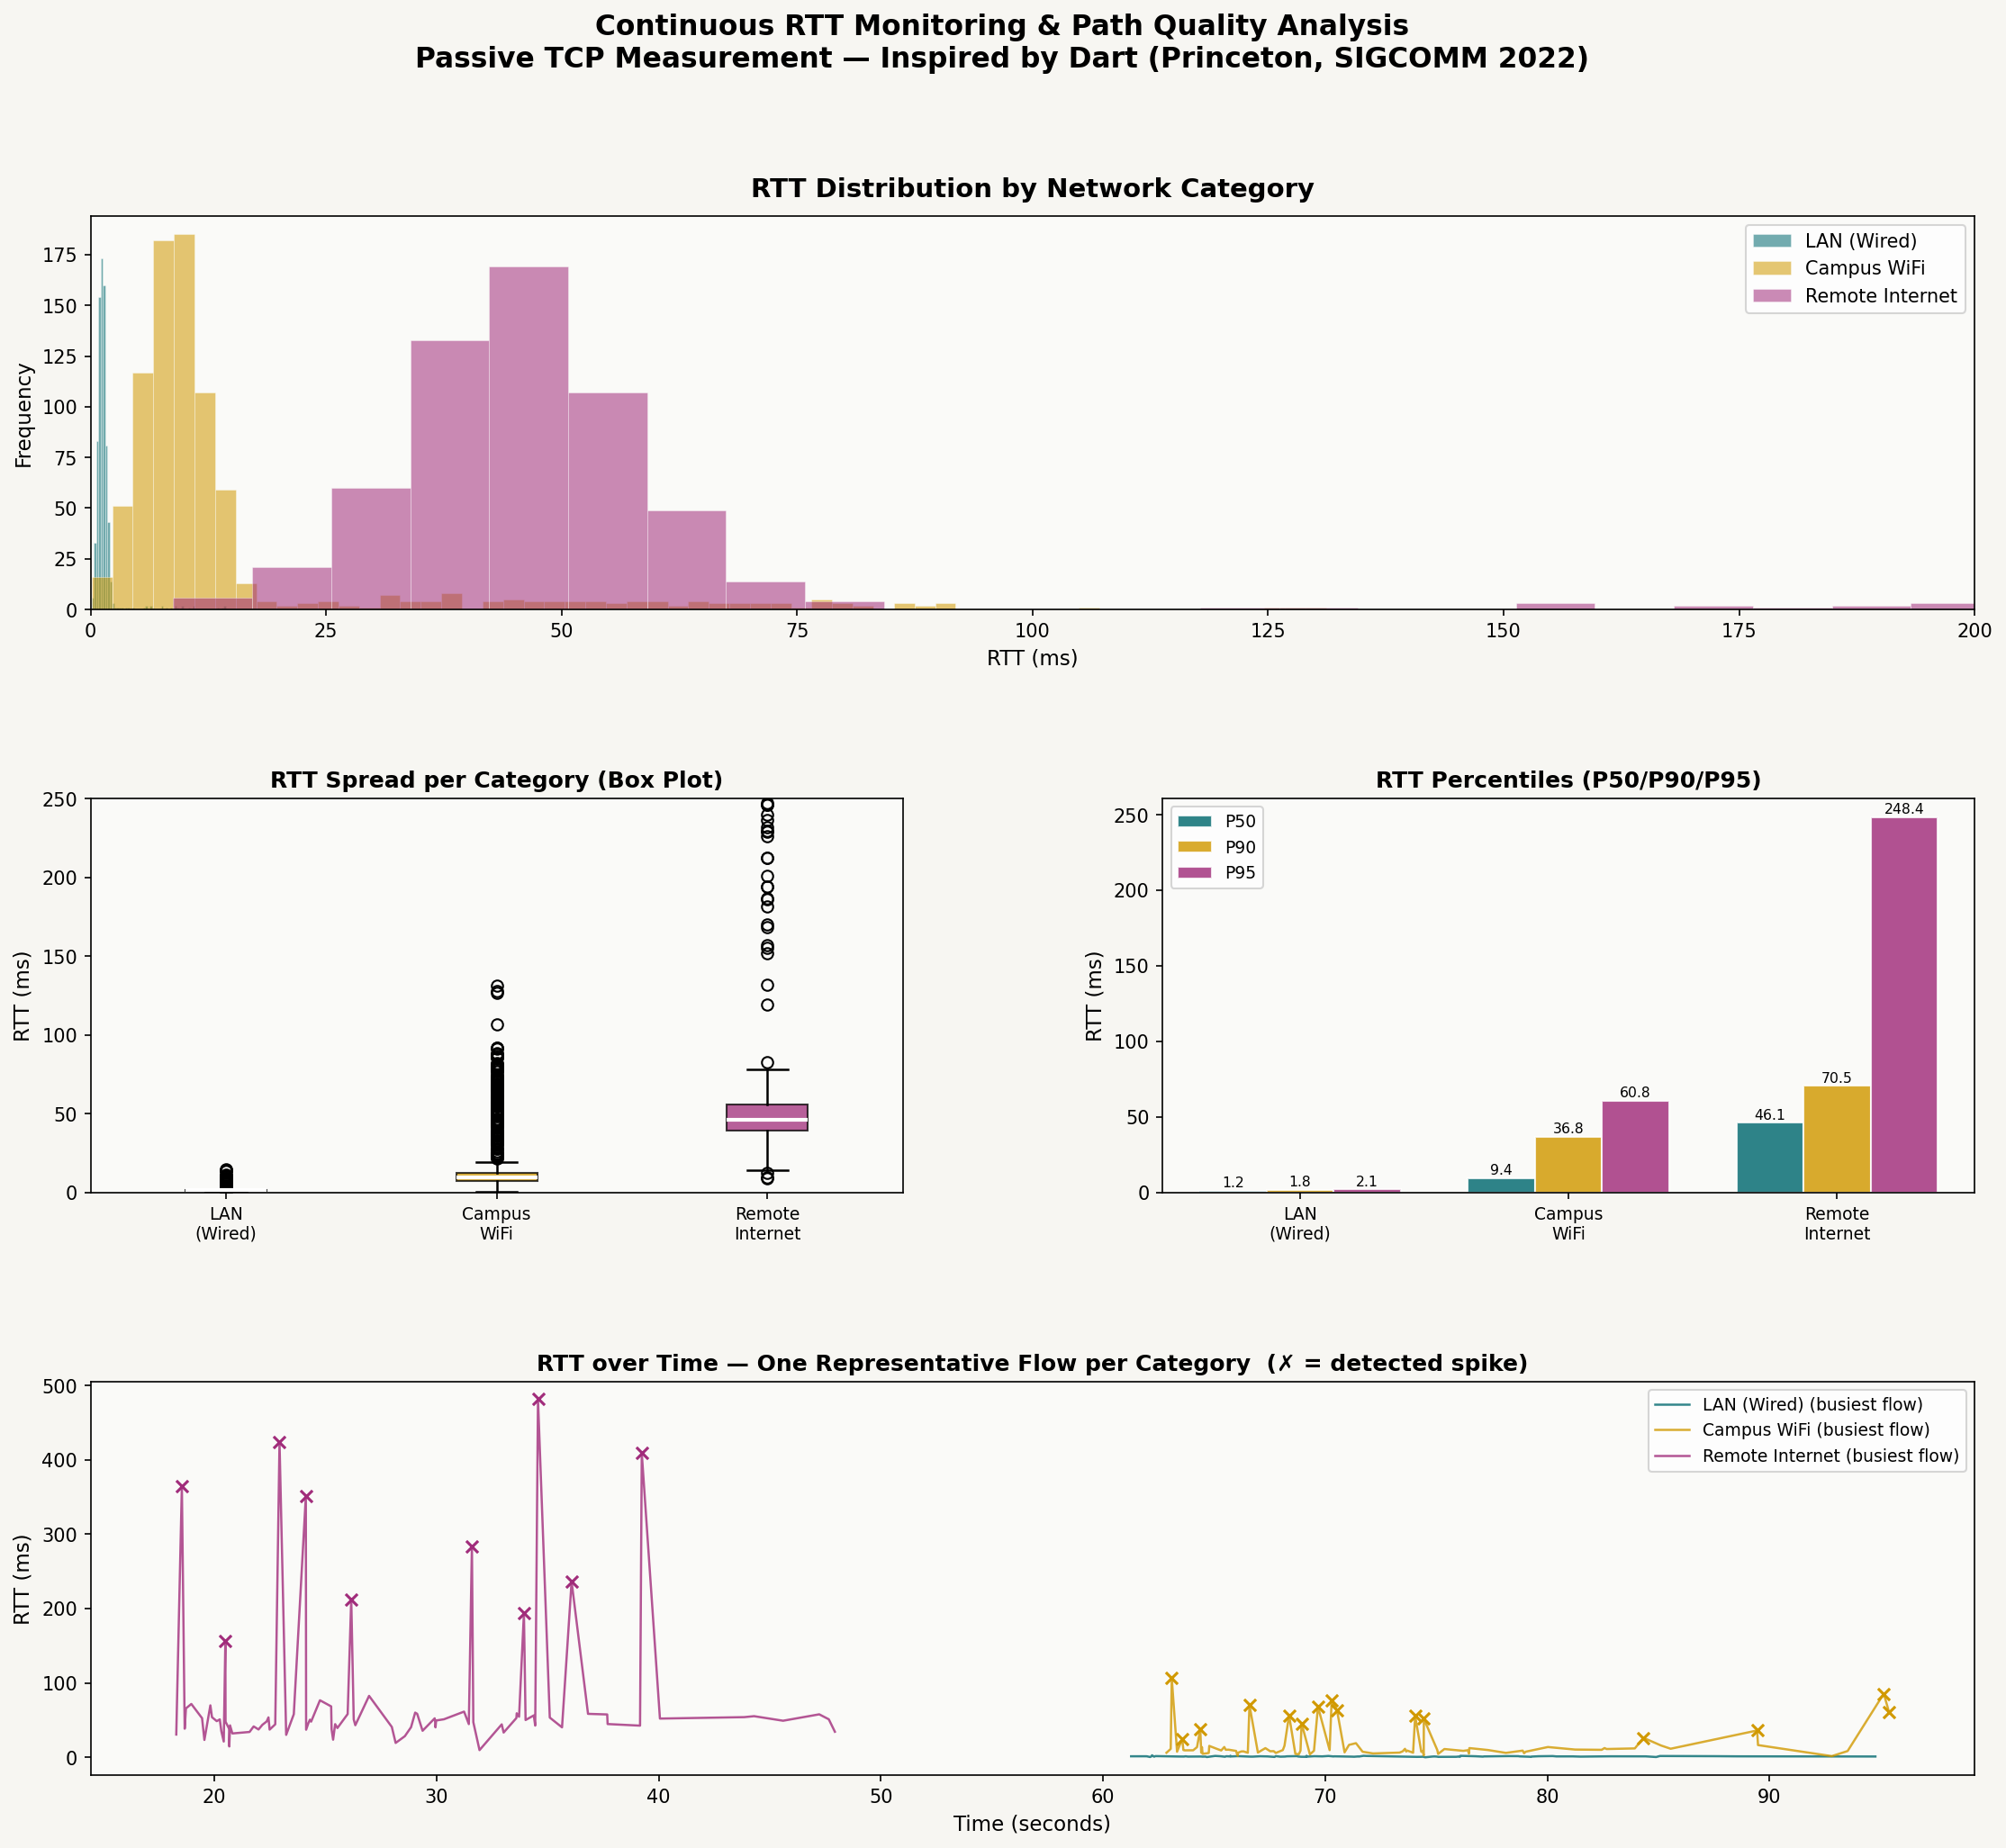
\includegraphics[width=\textwidth]{figures/v1_analysis.png}
    \caption{v1 RTT analysis --- live capture on college WiFi}
\end{figure}

\subsection{v2 Results}

\begin{table}[H]
    \centering
    \caption{v2 per-category RTT summary (all values in ms)}
    \begin{tabular}{lrrrrrr}
        \toprule
        \textbf{Category} & \textbf{N} & \textbf{Mean} & \textbf{P50} & \textbf{P90} & \textbf{P95} & \textbf{Max} \\
        \midrule
        HTTPS (Port 443) & 240 & 30.442 & 0.211 & 64.088  & 289.061 & 431.096 \\
        Unknown TCP      & 7   & 7.817  & 0.105 & 23.179  & 34.833  & 46.487  \\
        \bottomrule
    \end{tabular}
\end{table}

\noindent
\textbf{Methods used:} DATA-ACK = 236 samples, SYN-SYNACK = 11 samples.

\begin{figure}[H]
    \centering
    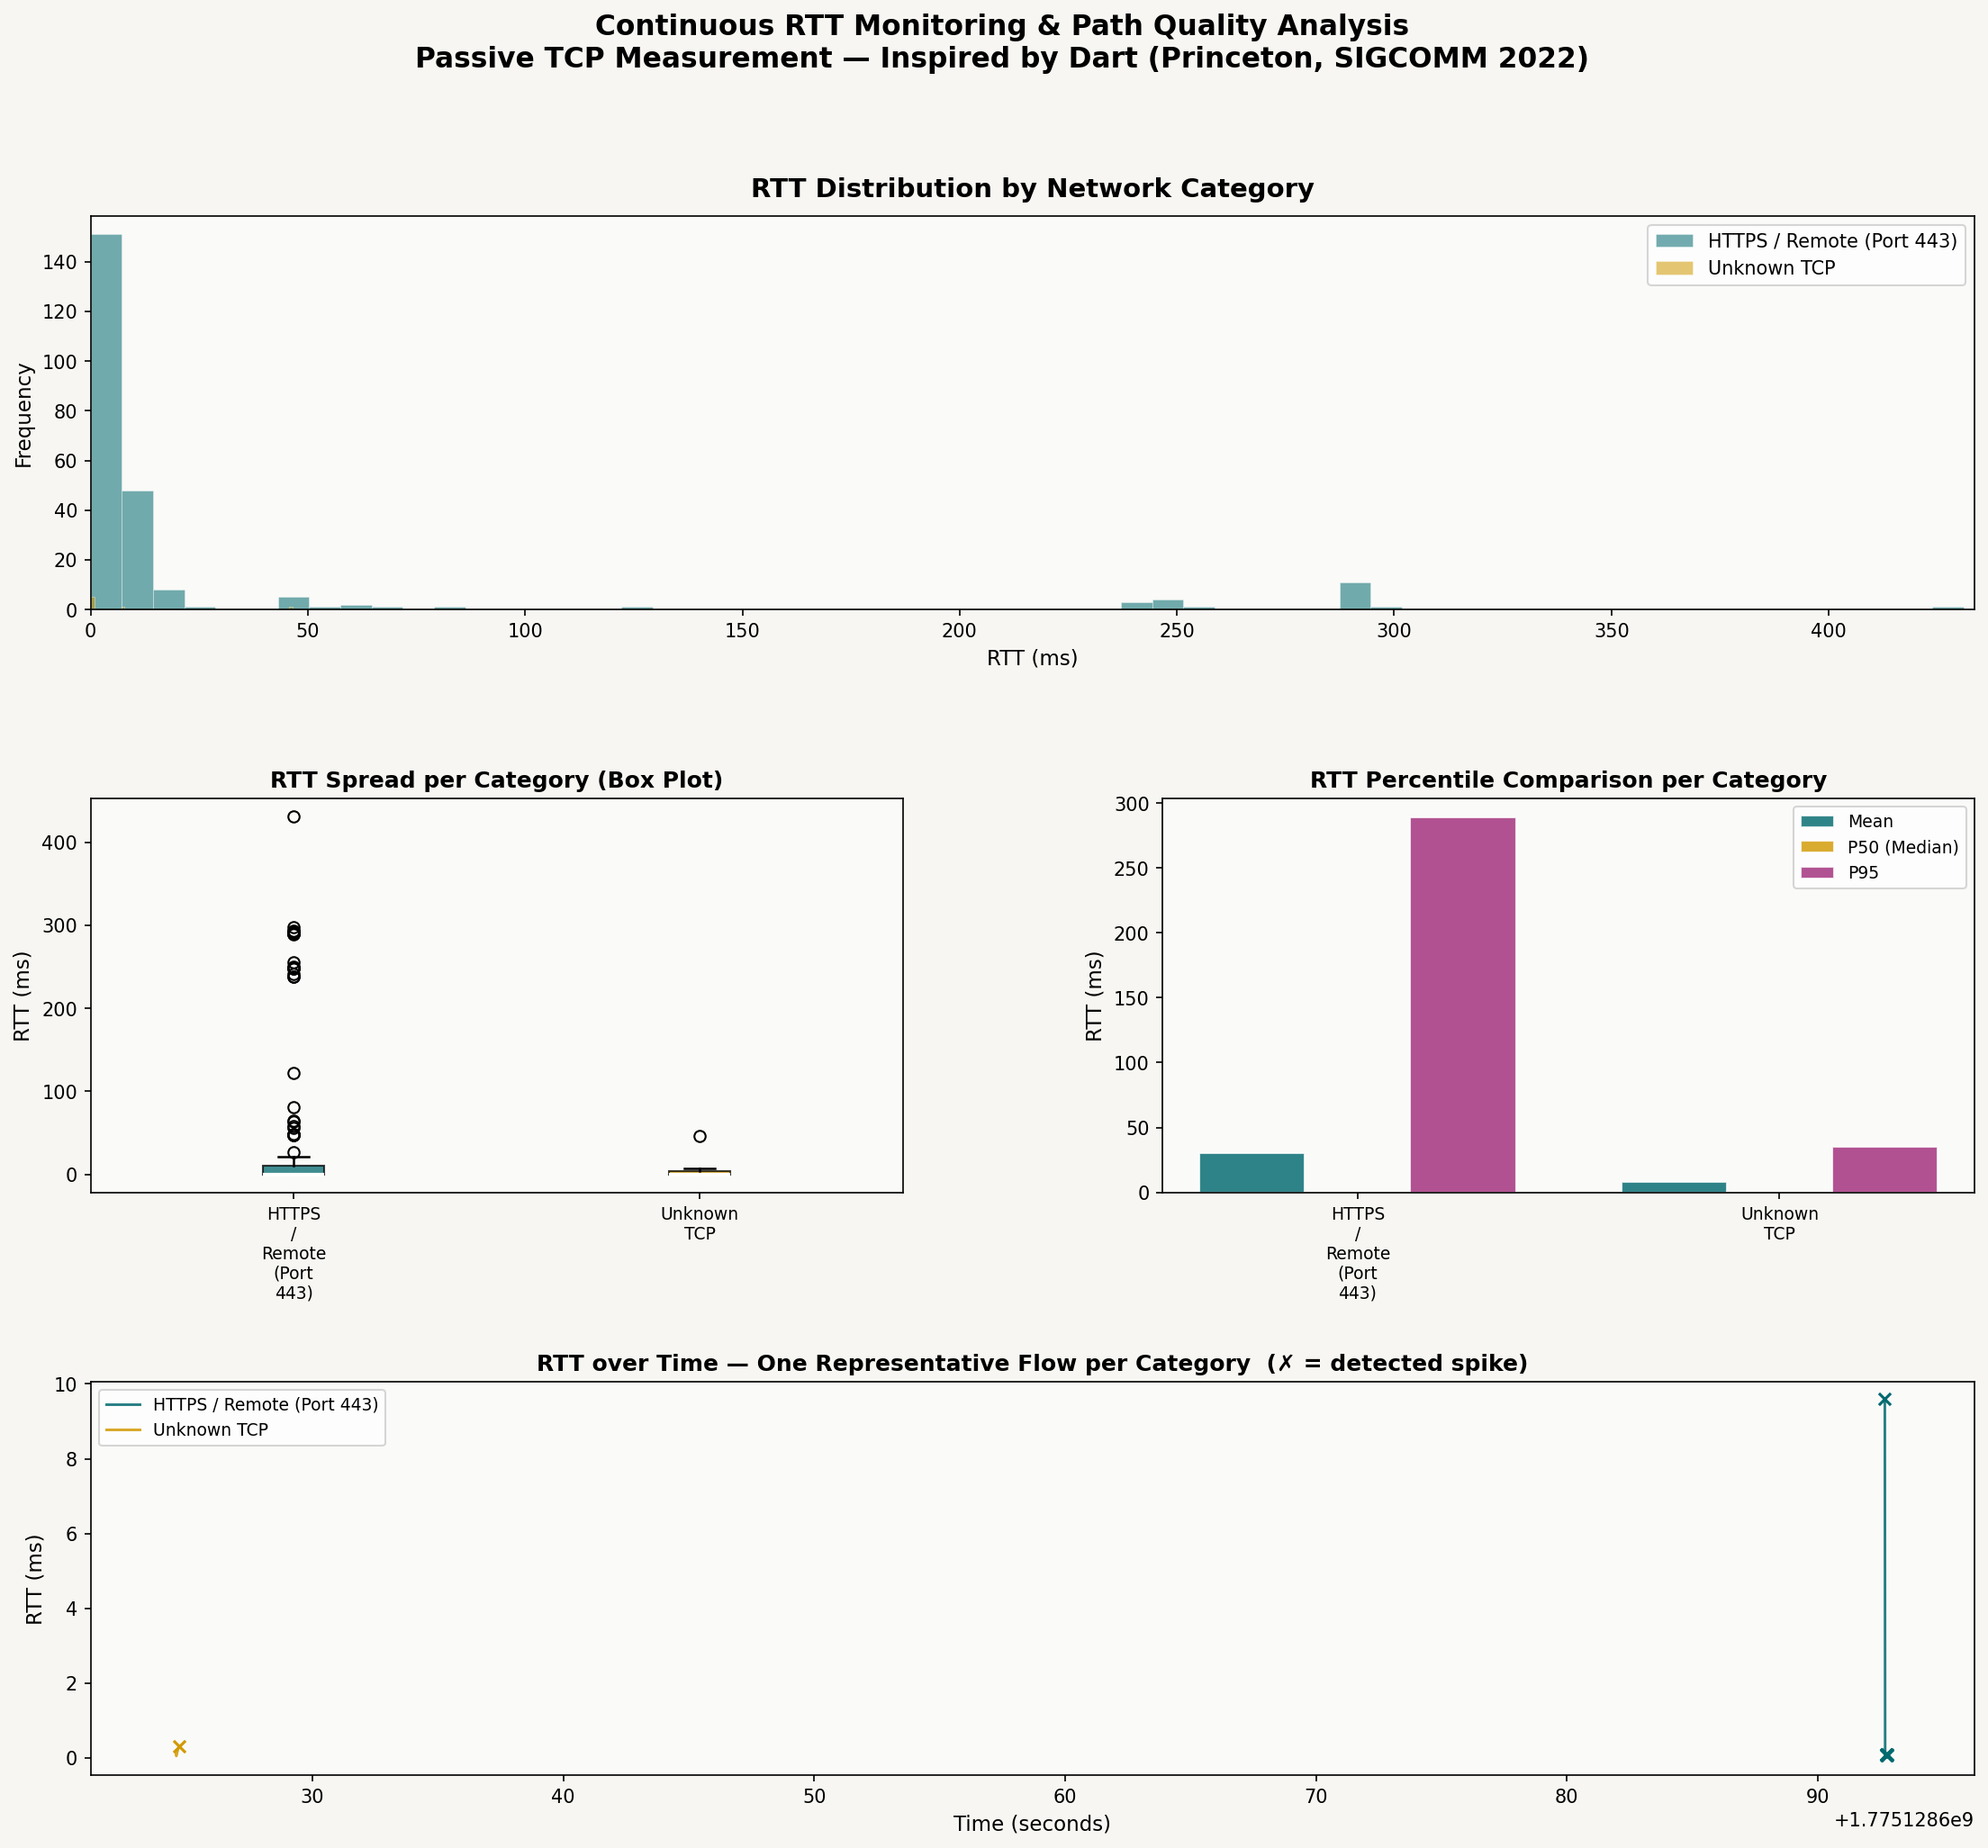
\includegraphics[width=\textwidth]{figures/v2_analysis.png}
    \caption{v2 RTT analysis --- offline pcap file}
\end{figure}

\subsection{v3 Results}

\begin{table}[H]
    \centering
    \caption{v3 per-window RTT summary (all values in ms)}
    \begin{tabular}{lrrrrr}
        \toprule
        \textbf{Window} & \textbf{N} & \textbf{Mean} & \textbf{P50} & \textbf{P90} & \textbf{Max} \\
        \midrule
        t = 5.3s  & 2  & 0.29 & 0.29 & 0.40  & 0.43  \\
        t = 12.2s & 76 & 1.92 & 0.55 & 5.92  & 13.46 \\
        t = 20.3s & 59 & 4.18 & 0.72 & 7.53  & 91.67 \\
        t = 36.2s & 28 & 2.23 & 0.85 & 6.81  & 9.97  \\
        t = 41.4s & 9  & 5.62 & 8.25 & 10.37 & 11.68 \\
        \bottomrule
    \end{tabular}
\end{table}

\begin{figure}[H]
    \centering
    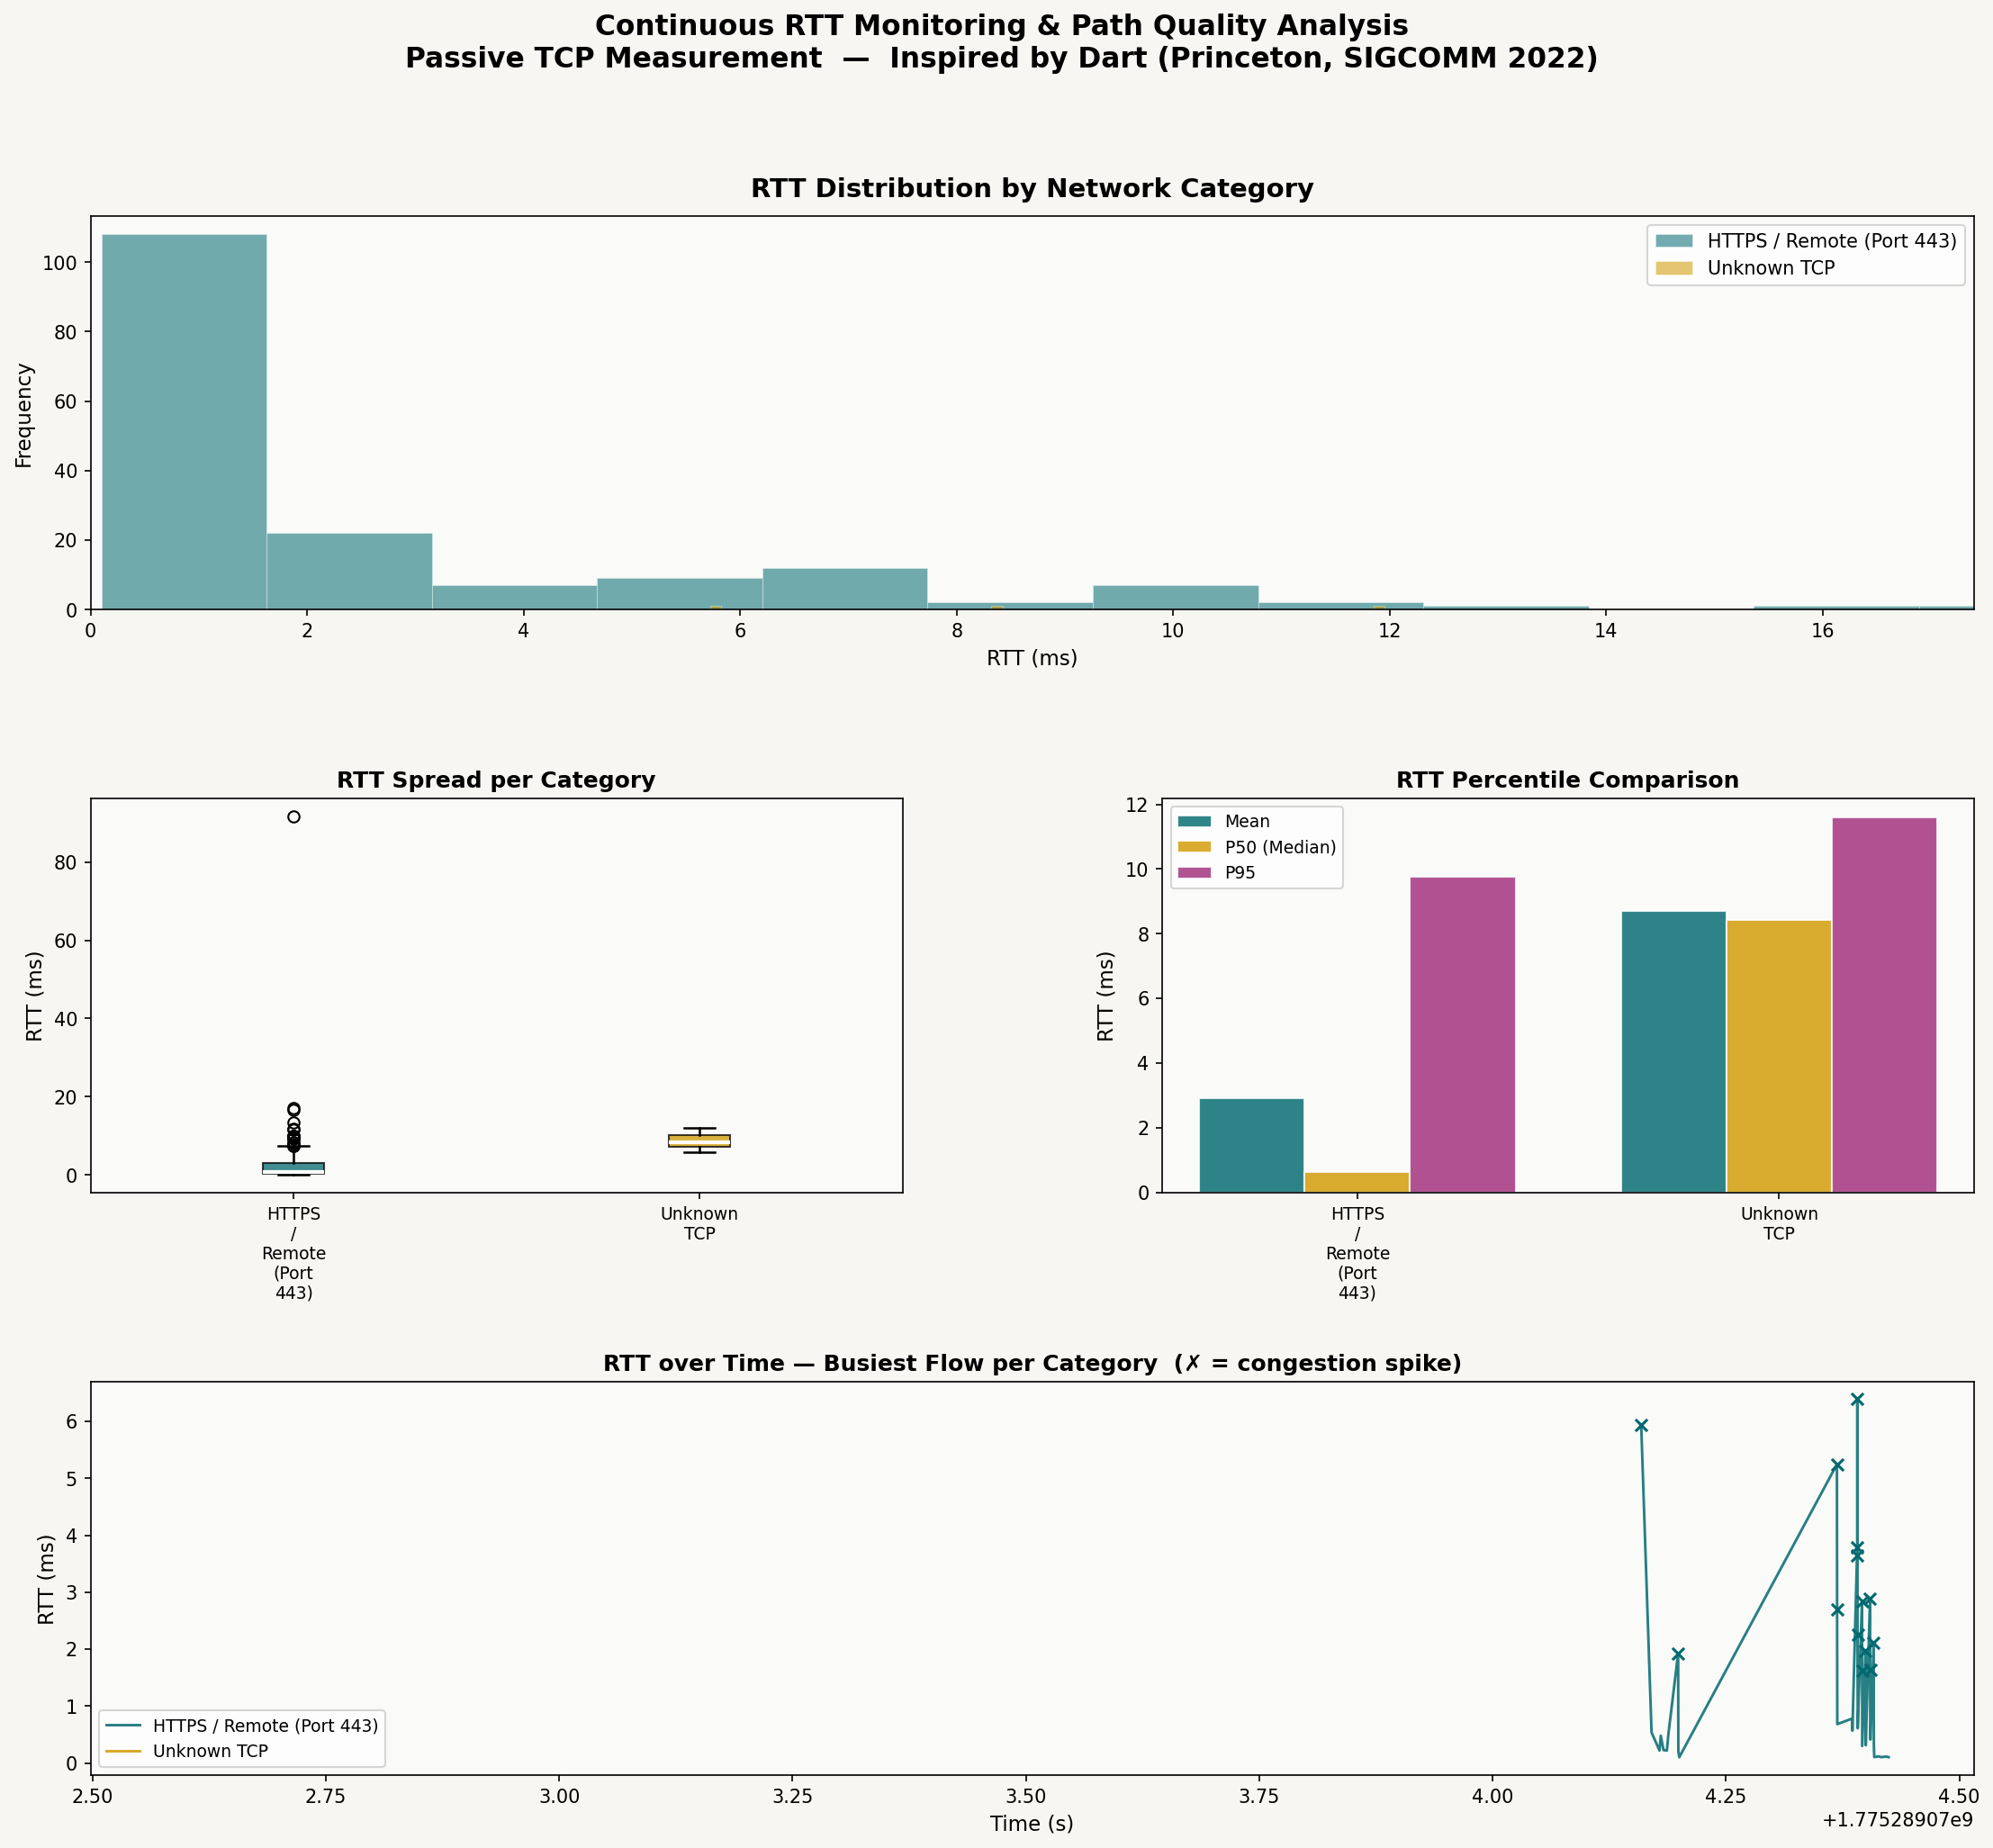
\includegraphics[width=\textwidth]{figures/v3_analysis.png}
    \caption{v3 RTT analysis --- configurable live monitor}
\end{figure}

\subsection{Observations}

\begin{itemize}[leftmargin=*]
    \item v1 clearly shows three latency tiers: LAN (1.4\,ms), WiFi (15\,ms), and Remote (66\,ms).
    \item v2 demonstrates that DATA-ACK increases flow coverage when handshakes are not captured.
    \item v3 provides interval-by-interval live feedback, enabling real-time network monitoring.
    \item The low P50 and higher Mean in v2 and v3 confirm a right-skewed RTT distribution.
    \item The 91.67\,ms spike at t\,=\,20s in v3 is an isolated outlier, not sustained congestion.
\end{itemize}

\section{Tools and Technologies}

\begin{table}[H]
    \centering
    \caption{Software stack}
    \begin{tabular}{lll}
        \toprule
        \textbf{Tool} & \textbf{Purpose} & \textbf{Notes} \\
        \midrule
        Python 3.10 & Core language         & mambaforge environment \\
        Scapy       & Packet sniffing       & Raw TCP/IP access \\
        pandas      & Aggregation, CSV      & groupby, percentiles \\
        NumPy       & Statistics            & P50, P90, P95 \\
        matplotlib  & Plot generation       & PNG charts \\
        Git/GitHub  & Version control       & Repository hosting \\
        \bottomrule
    \end{tabular}
\end{table}

\section{Conclusion}

The RTT Live Monitor successfully captures and analyses TCP Round-Trip Times in
real time with minimal overhead. The passive sniffing approach makes the tool
practical for real network environments as it does not inject additional traffic.

The development from v1 to v3 shows clear project progression: v1 built the
baseline live monitor, v2 added offline pcap analysis with dual RTT methods,
and v3 delivered a fully configurable and reliable live monitor suitable for
demonstration and final submission.

\subsection*{Future Extensions}
\begin{itemize}[leftmargin=*]
    \item Multi-interface monitoring across multiple NICs simultaneously
    \item Real-time anomaly alerting when P95 exceeds a configurable threshold
    \item Web-based dashboard for continuous network health visibility
    \item Support for IPv6 and QUIC/UDP-based RTT measurement
\end{itemize}

\section*{References}
\addcontentsline{toc}{section}{References}

\begin{thebibliography}{9}

\bibitem{cloudflare}
Cloudflare, \textit{What is Round-Trip Time (RTT)?},
\url{https://www.cloudflare.com/learning/cdn/glossary/round-trip-time-rtt/}

\bibitem{scapy}
Scapy Project, \textit{Scapy: Packet Manipulation Library},
\url{https://scapy.net}

\bibitem{pandas}
pandas Development Team, \textit{pandas.DataFrame.agg},
\url{https://pandas.pydata.org/docs/reference/api/pandas.DataFrame.agg.html}

\bibitem{dart}
S. Sengupta et al., \textit{Continuous In-Network Round-Trip Time Monitoring},
ACM SIGCOMM 2022,
\url{https://satadalsengupta.github.io/docs/papers/2022_sigcomm_dart.pdf}

\end{thebibliography}

\end{document}
